\emph{Pour $t \in [0~;~10]$, $f(t) = -25t^2 + 300t + 400$ où $t$ est le nombre de semaines écoulées
depuis le début de l'épidémie et $f(t)$ le nombre hebdomadaire de consultations.}

\subsection*{Partie A}

\begin{center}
	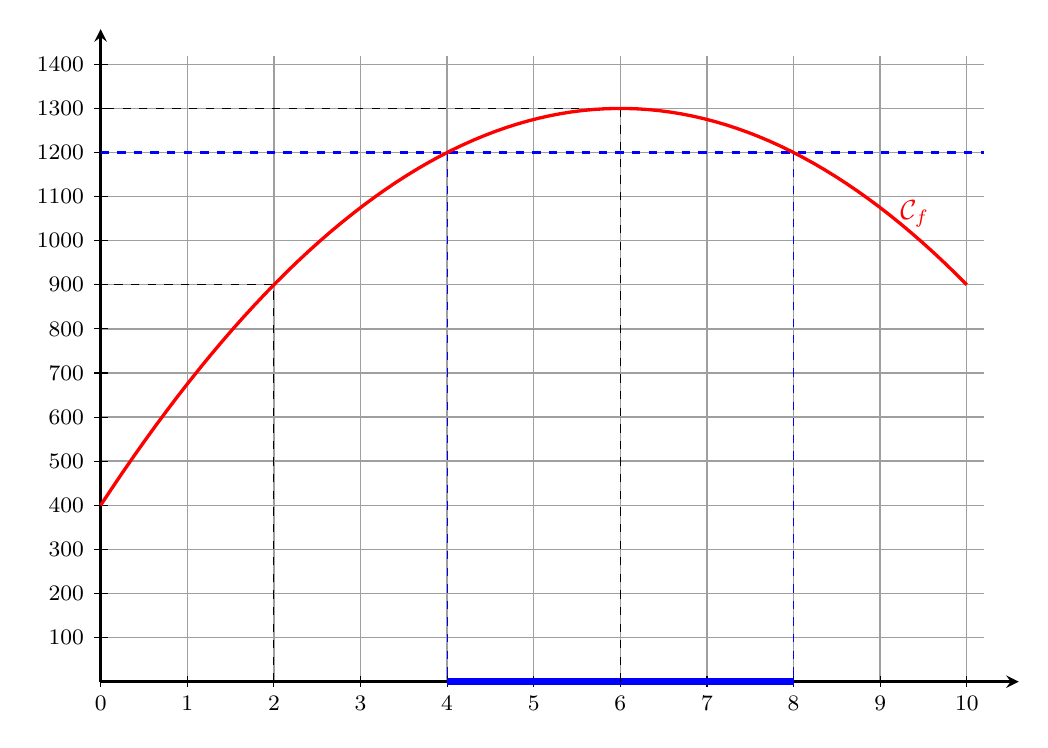
\begin{tikzpicture}[x=1.1cm,y=0.0056cm,>=stealth]
		\draw[xstep=1,ystep=100,gray!75,line width=0.5pt] (0,0) grid (10.2,1420);
		\draw[->,line width=1pt] (0,0) -- (10.6,0);
		\draw[->,line width=1pt] (0,0) -- (0,1480);
		\foreach \x in {0,1,...,10} \draw (\x,12) -- (\x,-12) node[below] {\footnotesize \np{\x}};
		\foreach \y in {100,200,...,1400} \draw (0.08,\y) -- (-0.08,\y) node[left] {\footnotesize \np{\y}};
		\draw[blue,dashed,line width=1pt] (0,1200) -- (10.2,1200);
		\draw[blue,dashed] (4,1200) -- (4,0);
		\draw[blue,dashed] (8,1200) -- (8,0);
		\draw[blue,line width=2.5pt] (4,0) -- (8,0);
		\draw[dashed] (2,0) -- (2,900) -- (0,900);
		\draw[dashed] (6,0) -- (6,1300) -- (0,1300);
		\draw[red,line width=1.2pt] plot[domain=0:10,samples=80] (\x,{-25*\x*\x+300*\x+400});
		\node[red] at (9.4,1060) {$\mathcal{C}_f$};
	\end{tikzpicture}
\end{center}

\begin{enumerate}
	\item Par lecture graphique, $f(2) \approx 900$.

	Deux semaines après le début de l'épidémie, il y a environ 900 consultations dans la
	semaine.

	\item La courbe coupe la droite d'équation $y = \np{1200}$ aux points d'abscisses 4 et 8, et se situe
	au-dessus entre ces deux valeurs.

	Le nombre de consultations dépasse \np{1200} pour $t \in \left]4~;~8\right[$, c'est-à-dire
	entre la 4\up{e} et la 8\up{e} semaine après le début de
	l'épidémie.

	\item Le sommet de la parabole a pour coordonnées $(6~;~\np{1300})$.

	Le nombre de consultations est maximal au bout de 6 semaines ; il atteint alors
	\np{1300} consultations dans la semaine.
\end{enumerate}

\subsection*{Partie B}

\begin{enumerate}
	\item $f(0) = -25\times 0^2 + 300\times 0 + 400 = 400$.

	Au début de l'épidémie, on compte 400 consultations dans la semaine.

	\item Pour tout réel $t$ de $[0~;~10]$,
$f'(t) = -25\times 2t + 300\times 1 + 0 = -50t + 300$.

	\item $f'(t) = 0 \iff -50t + 300 = 0 \iff -50t = -300 \iff t = \dfrac{-300}{-50} = 6$.
	
$S = \{6\}$.

	\item $f'(t) = -50t + 300$ est une expression affine de coefficient directeur $-50 < 0$ : elle est
	positive avant 6 et négative après.

	$f(0) = 400$, $f(6) = \np{1300}$ et
	$f(10) = -\np{2500} + \np{3000} + 400 = 900$.

	\begin{center}
		\begin{tikzpicture}
			\tkzTabInit[lgt=3.4,espcl=2.8]{$t$/1,$f'(t)$/1,$f$/2}{$0$,$6$,$10$}
			\tkzTabLine{,+,z,-,}
			\tkzTabVar{-/$400$,+/$\np{1300}$,-/$900$}
		\end{tikzpicture}
	\end{center}

	La fonction $f$ est croissante sur $[0~;~6]$ et décroissante sur $[6~;~10]$. Elle admet un
	maximum égal à \np{1300} en $t = 6$.
\end{enumerate}
